\documentclass[tikz, border=10pt]{standalone}
\usepackage{helvet}
\renewcommand{\familydefault}{\sfdefault}
\usepackage{tikz}
\usepackage{tikz-3dplot}
\usetikzlibrary{calc, arrows.meta, positioning, shapes.geometric, decorations.pathreplacing, 3d, fit, backgrounds}
\usepackage{amsmath}

% Define colors
\definecolor{emeraldpine}{HTML}{1A4D3E}
\definecolor{harvardcrimson}{HTML}{A51C30}
\definecolor{ethdarkblue}{HTML}{1F407A}
\definecolor{ethpetrol}{HTML}{007A87}
\definecolor{ethbronze}{HTML}{B87333}
\definecolor{ethpurple}{HTML}{5B4B8A}
\definecolor{ink}{HTML}{1A202C}
\definecolor{softink}{HTML}{4A5568}
\definecolor{paleink}{HTML}{A0AEC0}
\definecolor{cardbg}{HTML}{F8FAFC}
\definecolor{shadecolor}{HTML}{F4F6F9}

\begin{document}

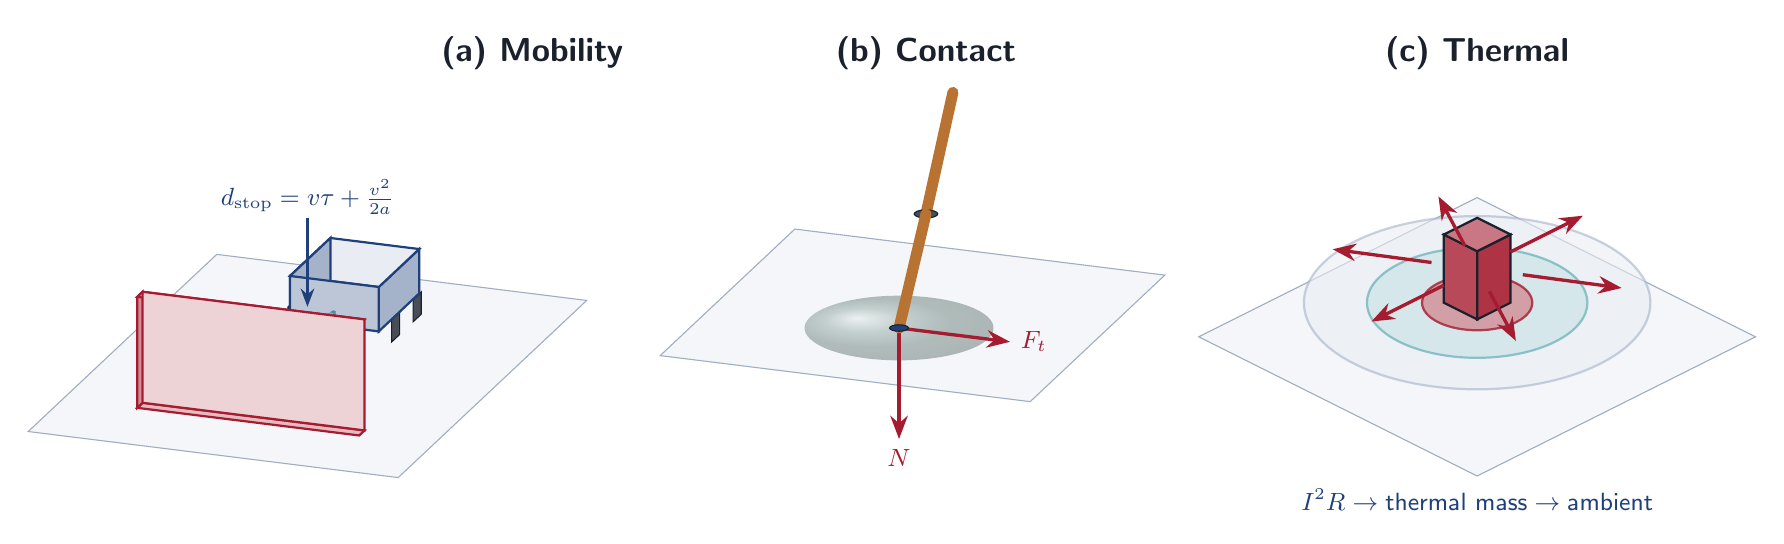
\begin{tikzpicture}[
    font=\sffamily,
    >=Stealth
]

% Panel dimensions and positions
\def\panelspacing{7}

% Panel A: Mobility
\begin{scope}[xshift=0, yshift=0]
    \node[anchor=north, font=\bfseries\large, text=ink] at (2, 3.5) {(a) Mobility};
    
    \tdplotsetmaincoords{70}{110}
    \begin{scope}[tdplot_main_coords, shift={(0, 0, 0)}]
        % Ground plane
        \fill[shadecolor, draw=paleink] (-1,-2.5,0) -- (6,-2.5,0) -- (6,2.5,0) -- (-1,2.5,0) -- cycle;
        
        % Wheels
        % Left side wheels (y=0.7) - further away
        \filldraw[fill=ink!80, draw=ink] (0.2, 0.7, 0) -- (0.5, 0.7, 0) -- (0.5, 0.7, 0.3) -- (0.2, 0.7, 0.3) -- cycle;
        \filldraw[fill=ink!80, draw=ink] (1.0, 0.7, 0) -- (1.3, 0.7, 0) -- (1.3, 0.7, 0.3) -- (1.0, 0.7, 0.3) -- cycle;
        % Right side wheels (y=-0.7) - closer
        \filldraw[fill=ink!80, draw=ink] (0.2, -0.7, 0) -- (0.5, -0.7, 0) -- (0.5, -0.7, 0.3) -- (0.2, -0.7, 0.3) -- cycle;
        \filldraw[fill=ink!80, draw=ink] (1.0, -0.7, 0) -- (1.3, -0.7, 0) -- (1.3, -0.7, 0.3) -- (1.0, -0.7, 0.3) -- cycle;

        % Robot base faces
        % Left face (y=0.6) (further)
        \filldraw[fill=ethdarkblue!40, draw=ethdarkblue, thick] (0,0.6,0.2) -- (0,0.6,0.8) -- (1.5,0.6,0.8) -- (1.5,0.6,0.2) -- cycle;
        % Top face (z=0.8)
        \filldraw[fill=ethdarkblue!10, draw=ethdarkblue, thick] (0,-0.6,0.8) -- (1.5,-0.6,0.8) -- (1.5,0.6,0.8) -- (0,0.6,0.8) -- cycle;
        % Right face (y=-0.6) (closer)
        \filldraw[fill=ethdarkblue!40, draw=ethdarkblue, thick] (0,-0.6,0.2) -- (0,-0.6,0.8) -- (1.5,-0.6,0.8) -- (1.5,-0.6,0.2) -- cycle;
        % Front face (x=1.5) (closest)
        \filldraw[fill=ethdarkblue!30, draw=ethdarkblue, thick] (1.5,-0.6,0.2) -- (1.5,-0.6,0.8) -- (1.5,0.6,0.8) -- (1.5,0.6,0.2) -- cycle;
        
        % Translucent stopping cone (blue)
        % Projecting forward along x axis from x=1.5 to x=4.5
        \fill[ethpetrol!30, opacity=0.4, draw=ethpetrol, dashed, thick] 
            (1.5, 0, 0.4) -- (4.5, -1.2, 0) -- (4.5, 1.2, 0) -- cycle;
        \fill[ethpetrol!40, opacity=0.5, draw=ethpetrol, dashed, thick] 
            (1.5, 0, 0.4) -- (4.5, 1.2, 0) -- (4.5, 1.2, 1.2) -- (4.5, -1.2, 1.2) -- (4.5, -1.2, 0) -- cycle;
            
        % Obstacle wall (at x=4.5)
        \filldraw[fill=harvardcrimson!30, draw=harvardcrimson, thick] (4.5,-1.5,0) -- (4.7,-1.5,0) -- (4.7,1.5,0) -- (4.5,1.5,0) -- cycle;
        \filldraw[fill=harvardcrimson!50, draw=harvardcrimson, thick] (4.5,-1.5,0) -- (4.5,-1.5,1.5) -- (4.7,-1.5,1.5) -- (4.7,-1.5,0) -- cycle;
        \filldraw[fill=harvardcrimson!40, draw=harvardcrimson, thick] (4.5,-1.5,1.5) -- (4.7,-1.5,1.5) -- (4.7,1.5,1.5) -- (4.5,1.5,1.5) -- cycle;
        \filldraw[fill=harvardcrimson!20, draw=harvardcrimson, thick] (4.5,-1.5,1.5) -- (4.5,1.5,1.5) -- (4.5,1.5,0) -- (4.5,-1.5,0) -- cycle;

        % Label
        \draw[<-, thick, ethdarkblue] (2.5, 0, 0.8) -- (2.5, 0, 2) node[above, font=\small, fill=white, inner sep=1pt] {$d_{\mathrm{stop}} = v\tau + \frac{v^2}{2a}$};
    \end{scope}
\end{scope}

% Panel B: Contact
\begin{scope}[xshift=\panelspacing cm, yshift=0]
    \node[anchor=north, font=\bfseries\large, text=ink] at (0, 3.5) {(b) Contact};
    
    \tdplotsetmaincoords{70}{110}
    \begin{scope}[tdplot_main_coords, shift={(0, 0, 0)}]
        % Base plane (workpiece)
        \filldraw[fill=shadecolor, draw=paleink] (-2,-2.5,0) -- (3,-2.5,0) -- (3,2.5,0) -- (-2,2.5,0) -- cycle;
        
        % Impedance dome (translucent green/emeraldpine) - drawn first so it's behind arm
        \shade[ball color=emeraldpine, opacity=0.3] (1,0,0) circle (1.2);
        
        % Force vectors
        \draw[->, very thick, harvardcrimson] (1,0,0) -- (1,0,-1.5) node[below, font=\small] {$N$};
        \draw[->, very thick, harvardcrimson] (1,0,0) -- (1,1.5,0) node[right, font=\small] {$F_t$};

        % Robot arm
        % Base link and joint
        \draw[ethbronze, line width=4pt, line cap=round] (-1,0,2.5) -- (0,0,1.2);
        \filldraw[fill=ink!80, draw=ink] (0,0,1.2) circle (0.15);
        \draw[ethbronze, line width=4pt, line cap=round] (0,0,1.2) -- (1,0,0);
        
        % End effector
        \filldraw[fill=ethdarkblue, draw=ink] (1,0,0) circle (0.12);
        
    \end{scope}
\end{scope}

% Panel C: Thermal/Flow
\begin{scope}[xshift=2*\panelspacing cm, yshift=0]
    \node[anchor=north, font=\bfseries\large, text=ink] at (0, 3.5) {(c) Thermal};
    
    \tdplotsetmaincoords{60}{135}
    \begin{scope}[tdplot_main_coords, shift={(0, 0, 0)}]
        
        % Background plane to match others
        \filldraw[fill=shadecolor, draw=paleink] (-2.5,-2.5,-0.5) -- (2.5,-2.5,-0.5) -- (2.5,2.5,-0.5) -- (-2.5,2.5,-0.5) -- cycle;

        % Outer cool zone
        \filldraw[fill=ethdarkblue!10, draw=ethdarkblue!40, thick, opacity=0.6] (0,0,0) circle (2.2);
        
        % Mid zone
        \filldraw[fill=ethpetrol!20, draw=ethpetrol!60, thick, opacity=0.7] (0,0,0) circle (1.4);
        
        % Inner hot zone (stator/battery)
        \filldraw[fill=harvardcrimson!50, draw=harvardcrimson, thick, opacity=0.8] (0,0,0) circle (0.7);
        
        % Motor/battery solid box
        % Back faces (not drawn, solid box)
        % Bottom (z=0), Top (z=1), Front (x=-0.3), Back (x=0.3), Left (y=-0.3), Right (y=0.3)
        % For 60, 135: camera is looking from x>0, y>0, z>0
        % Visible faces: Top (z=1), Right (y=0.3), Back? Actually 135 deg means looking from positive x and positive y.
        % So visible faces: x=0.3 (front-ish), y=0.3 (right-ish), z=1 (top)
        \filldraw[fill=harvardcrimson!80, draw=ink, thick] (0.3,-0.3,0) -- (0.3,0.3,0) -- (0.3,0.3,1) -- (0.3,-0.3,1) -- cycle; % x=0.3
        \filldraw[fill=harvardcrimson!90, draw=ink, thick] (-0.3,0.3,0) -- (0.3,0.3,0) -- (0.3,0.3,1) -- (-0.3,0.3,1) -- cycle; % y=0.3
        \filldraw[fill=harvardcrimson!60, draw=ink, thick] (-0.3,-0.3,1) -- (0.3,-0.3,1) -- (0.3,0.3,1) -- (-0.3,0.3,1) -- cycle; % z=1
        
        % Heat flux arrows (radiating)
        % Draw them slightly elevated (z=0.5)
        \foreach \ang in {0, 60, 120, 180, 240, 300} {
            \draw[->, very thick, harvardcrimson] ({0.6*cos(\ang)}, {0.6*sin(\ang)}, 0.5) -- ({1.9*cos(\ang)}, {1.9*sin(\ang)}, 0.5);
        }
        
    \end{scope}
    
    % Label
    \node[font=\small, align=center, ethdarkblue, fill=white, fill opacity=0.9, text opacity=1, inner sep=2pt] at (0, -2.5) {$I^2R \rightarrow \text{thermal mass} \rightarrow \text{ambient}$};
\end{scope}

\end{tikzpicture}
\end{document}
